\section*{Physical Parameter Analysis and Model Calibration}

We adopt a consistent set of physical parameters for both the full-scale femur simulations and the box-shaped verification tests used for convergence studies. Unless stated otherwise, we report length in [mm], time in [day], stress/energy in [MPa], and density in [g/cm$^3$].

\paragraph{Mechanical (elasticity) parameters.}
The density--elasticity law uses $E_0=7500\,\mathrm{MPa}$ ($7.5\,\mathrm{GPa}$), $\nu_0=0.3$, and a smooth exponent transition from $n_{\mathrm{trab}}=2.0$ to $n_{\mathrm{cort}}=1.3$ over the density interval $[\rho_{\mathrm{trab}}^{\max},\rho_{\mathrm{cort}}^{\min}]$ with $\rho_{\mathrm{trab}}^{\max}=1.0\,\mathrm{g/cm^3}$ and $\rho_{\mathrm{cort}}^{\min}=1.25\,\mathrm{g/cm^3}$. We use the reference density $\rho_{\mathrm{ref}}=1.0\,\mathrm{g/cm^3}$ in the power law and the smooth lower clamp $\rho_{\min}=0.1\,\mathrm{g/cm^3}$. Fabric-guided directional scaling uses stiffness exponents $p_E=1.0$ (axial) and $p_G=1.0$ (shear), with eigenvalue-ratio bounds $m_{\min}=0.2$ and $m_{\max}=5.0$.

\paragraph{Stimulus (mechanoregulation) parameters.}
The cycle-weighted power mean in \eqref{eq:stim-psi-nd} uses exponent $p=4.0$. The mechanostat is parametrized by $\psi_{\mathrm{ref}}=0.01\,\mathrm{MPa}$ and the specific-energy reference $m_{\mathrm{ref}}=\psi_{\mathrm{ref}}/\rho_{\mathrm{ref}}$ with $\rho_{\mathrm{ref}}=1.0\,\mathrm{g/cm^3}$. The diffusion--reaction constants are $\tau_S=25\,\mathrm{day}$ and $D_S=1.0\,\mathrm{mm^2/day}$, and the dimensionless saturation/lazy-zone parameters are $S_{\max}=1.0$, $\kappa_S=0.5$, and $\delta_0=0.10$.

\paragraph{Density-evolution parameters.}
The density bounds and initialization are $\rho_{\min}=0.1\,\mathrm{g/cm^3}$, $\rho_{\max}=2.0\,\mathrm{g/cm^3}$, and $\rho_0=1.0\,\mathrm{g/cm^3}$, with reference density $\rho_{\mathrm{ref}}=1.0\,\mathrm{g/cm^3}$. Formation and resorption gains are $k_{\mathrm{form}}=k_{\mathrm{res}}=2\times 10^{-2}\,\mathrm{g/cm^3/day}$, and the isotropic density diffusion coefficient is $D_\rho=2\times 10^{-2}\,\mathrm{mm^2/day}$. The surface-availability factor $A_{\mathrm{surf}}$ is enabled in the results below and uses $\rho_{\mathrm{tissue}}=2.0\,\mathrm{g/cm^3}$, $A_{\min}=0.02$ (dimensionless), and $S_0=1.0\,\mathrm{mm^{-1}}$.

\paragraph{Fabric-evolution parameters.}
The log-fabric equation \eqref{eq:L-strong-nd} uses $\tau_A=50\,\mathrm{day}$, $D_A=1.0\,\mathrm{mm^2/day}$, and capacity $c_A=1.0$ (dimensionless). The target construction \eqref{eq:M-hat-nd} uses exponent $\gamma_F=1.0$, diagonal regularization $\varepsilon_Q=10^{-12}\,\mathrm{MPa^2}$ (added to $\bar{\mathbf Q}$), and eigenvalue-ratio bounds $m_{\min}=0.2$ and $m_{\max}=5.0$. The activity gate uses $\varepsilon_a=10^{-4}$.

\paragraph{Linear and coupling solver parameters.}
Each linear subproblem is solved by a Krylov method with GAMG preconditioning and tolerances $\mathrm{rtol}=10^{-7}$, $\mathrm{atol}=10^{-8}$, and $\mathrm{it}_{\max}=200$. The mechanics block uses GMRES with GAMG and Chebyshev smoothing; the transport-type blocks (stimulus, density, and fabric) use the configured Krylov type (default MINRES) with GAMG. Nonlinear coupling at a fixed time level uses block Gauss--Seidel with Anderson acceleration (enabled in all results below): history length $m=4$, mixing $\beta=1.0$, and scaled Tikhonov regularization $\lambda=10^{-2}$; the step limiter uses $c_{\mathrm{step}}=1.5$. History restarts use stall ratio $\chi_{\mathrm{stall}}=1.10$ with window $w=2$ and patience $k_{\mathrm{stall}}=2$, and a conditioning threshold $\kappa_{\max}=10^{5}$. The fixed-point stopping criterion is $r_{\mathrm{Pic}}\le \mathrm{tol}$ with $\mathrm{tol}=10^{-6}$ and a cap of $N_{\max}=25$ subiterations; optional outer-stall early abort uses $(W,\delta,P)=(8,0.05,2)$.

\paragraph{Time stepping and numerics.}
We advance from $t^0=0$ to $T$ using Backward--Euler with step sizes $\Delta t^n=t^{n+1}-t^n$ (constant $\Delta t^n\equiv \Delta t^0$ when adaptive control is disabled, except for the final truncation to hit $T$). When adaptive control is enabled, each \emph{attempted} step uses an explicit Adams--Bashforth predictor as an initial guess for the coupled implicit solve on $\mathbf{x}=(\mathbf L,S,\rho)$. Let $\mathbf{x}^n$ denote the last accepted state and let $\dot{\mathbf x}^{n}\approx (\mathbf{x}^n-\mathbf{x}^{n-1})/\Delta t^{n-1}$ be the stored discrete rate (updated only after accepted steps). With step ratio $r_n=\Delta t^n/\Delta t^{n-1}$, the AB2 predictor reads
\begin{equation}\label{eq:ab2-predict}
\mathbf{x}_{\mathrm{pred}}^{n+1}
=\mathbf{x}^n+\Delta t^n\left(\left(1+\tfrac12 r_n\right)\dot{\mathbf x}^{n}-\tfrac12 r_n\,\dot{\mathbf x}^{n-1}\right),
\end{equation}
and falls back to AB1 (or constant prediction on the very first step) when insufficient history is available. Starting from $\mathbf{x}_{\mathrm{pred}}^{n+1}$ we solve the coupled Backward--Euler problem at $t^{n+1}$ by the fixed-point scheme in \S\ref{sec:fp-aa}, yielding the corrected state $\mathbf{x}^{n+1}$. We estimate the time-discretization error by a global weighted RMS norm of the predictor--corrector difference,
\begin{equation}\label{eq:wrms-error}
e^{n+1}
=\left(\frac{1}{N_{\mathrm{tot}}}\sum_{i=1}^{N_{\mathrm{tot}}}
\left(\frac{x_i^{n+1}-x_{\mathrm{pred},i}^{n+1}}{\mathrm{rtol}_t\max(|x_i^{n+1}|,|x_{\mathrm{pred},i}^{n+1}|)+\mathrm{atol}_t}\right)^{\!2}\right)^{\!1/2},
\end{equation}
where the sum runs over all DOFs of $(\mathbf L,S,\rho)$ (global across MPI ranks) and $N_{\mathrm{tot}}$ is the total number of those DOFs. The adaptive controller is parametrized by $(\mathrm{rtol}_t,\mathrm{atol}_t)$, timestep bounds $(\Delta t_{\min},\Delta t_{\max})$, a safety factor $\eta$, shrink/growth limits $(g_{\min},g_{\max})$, and gains $(k_{\mathrm{exp}},k_P,k_I)$. A step is rejected if the coupled solve does not converge, or if $e^{n+1}>1$ (except that the first step is always accepted and, if $e^{1}>1$, only the \emph{next} timestep is reduced using the same shrink formula). On rejection we roll back to $\mathbf{x}^n$ and retry with a smaller timestep. For time-error rejections we use the shrink formula
\[
\Delta t^n \leftarrow \Delta t^n\cdot \min\!\left(0.9,\ \max\!\left(g_{\min},\ \eta\,(1/e^{n+1})^{1/k_{\mathrm{exp}}}\right)\right),
\]
whereas coupling failures trigger an immediate cut $\Delta t^n\leftarrow g_{\min}\Delta t^n$ and reset the AB history. For accepted steps with $n\ge1$ and $e^{n+1}\le 1$ we update the \emph{next} timestep by a Gustafsson PI controller:
\[
\Delta t^{n+1} \leftarrow \Delta t^n\cdot \min\!\left(g_{\max},\ \max\!\left(g_{\min},\ \eta\,(e^{n+1})^{-k_I}\left(\frac{e^{n}}{e^{n+1}}\right)^{k_P}\right)\right),
\]
with an I-only variant on the second accepted step; if $e^{n+1}<0.5$ we additionally prevent accidental shrink by enforcing the factor to be at least $1$. Finally, $\Delta t^n$ is clamped to $[\Delta t_{\min},\Delta t_{\max}]$ after each update; \cref{fig:time-adaptivity-controller} shows a diagnostic summary of the resulting controller behavior. Smooth clamps/splits use a global smoothing width $\varepsilon=10^{-6}$ (interpreted in the units of the smoothed quantity), and numerical integration uses quadrature degree $q=4$.

\begin{figure}[htbp]
  \centering
  \IfFileExists{images/time_adaptivity_demo.png}{%
    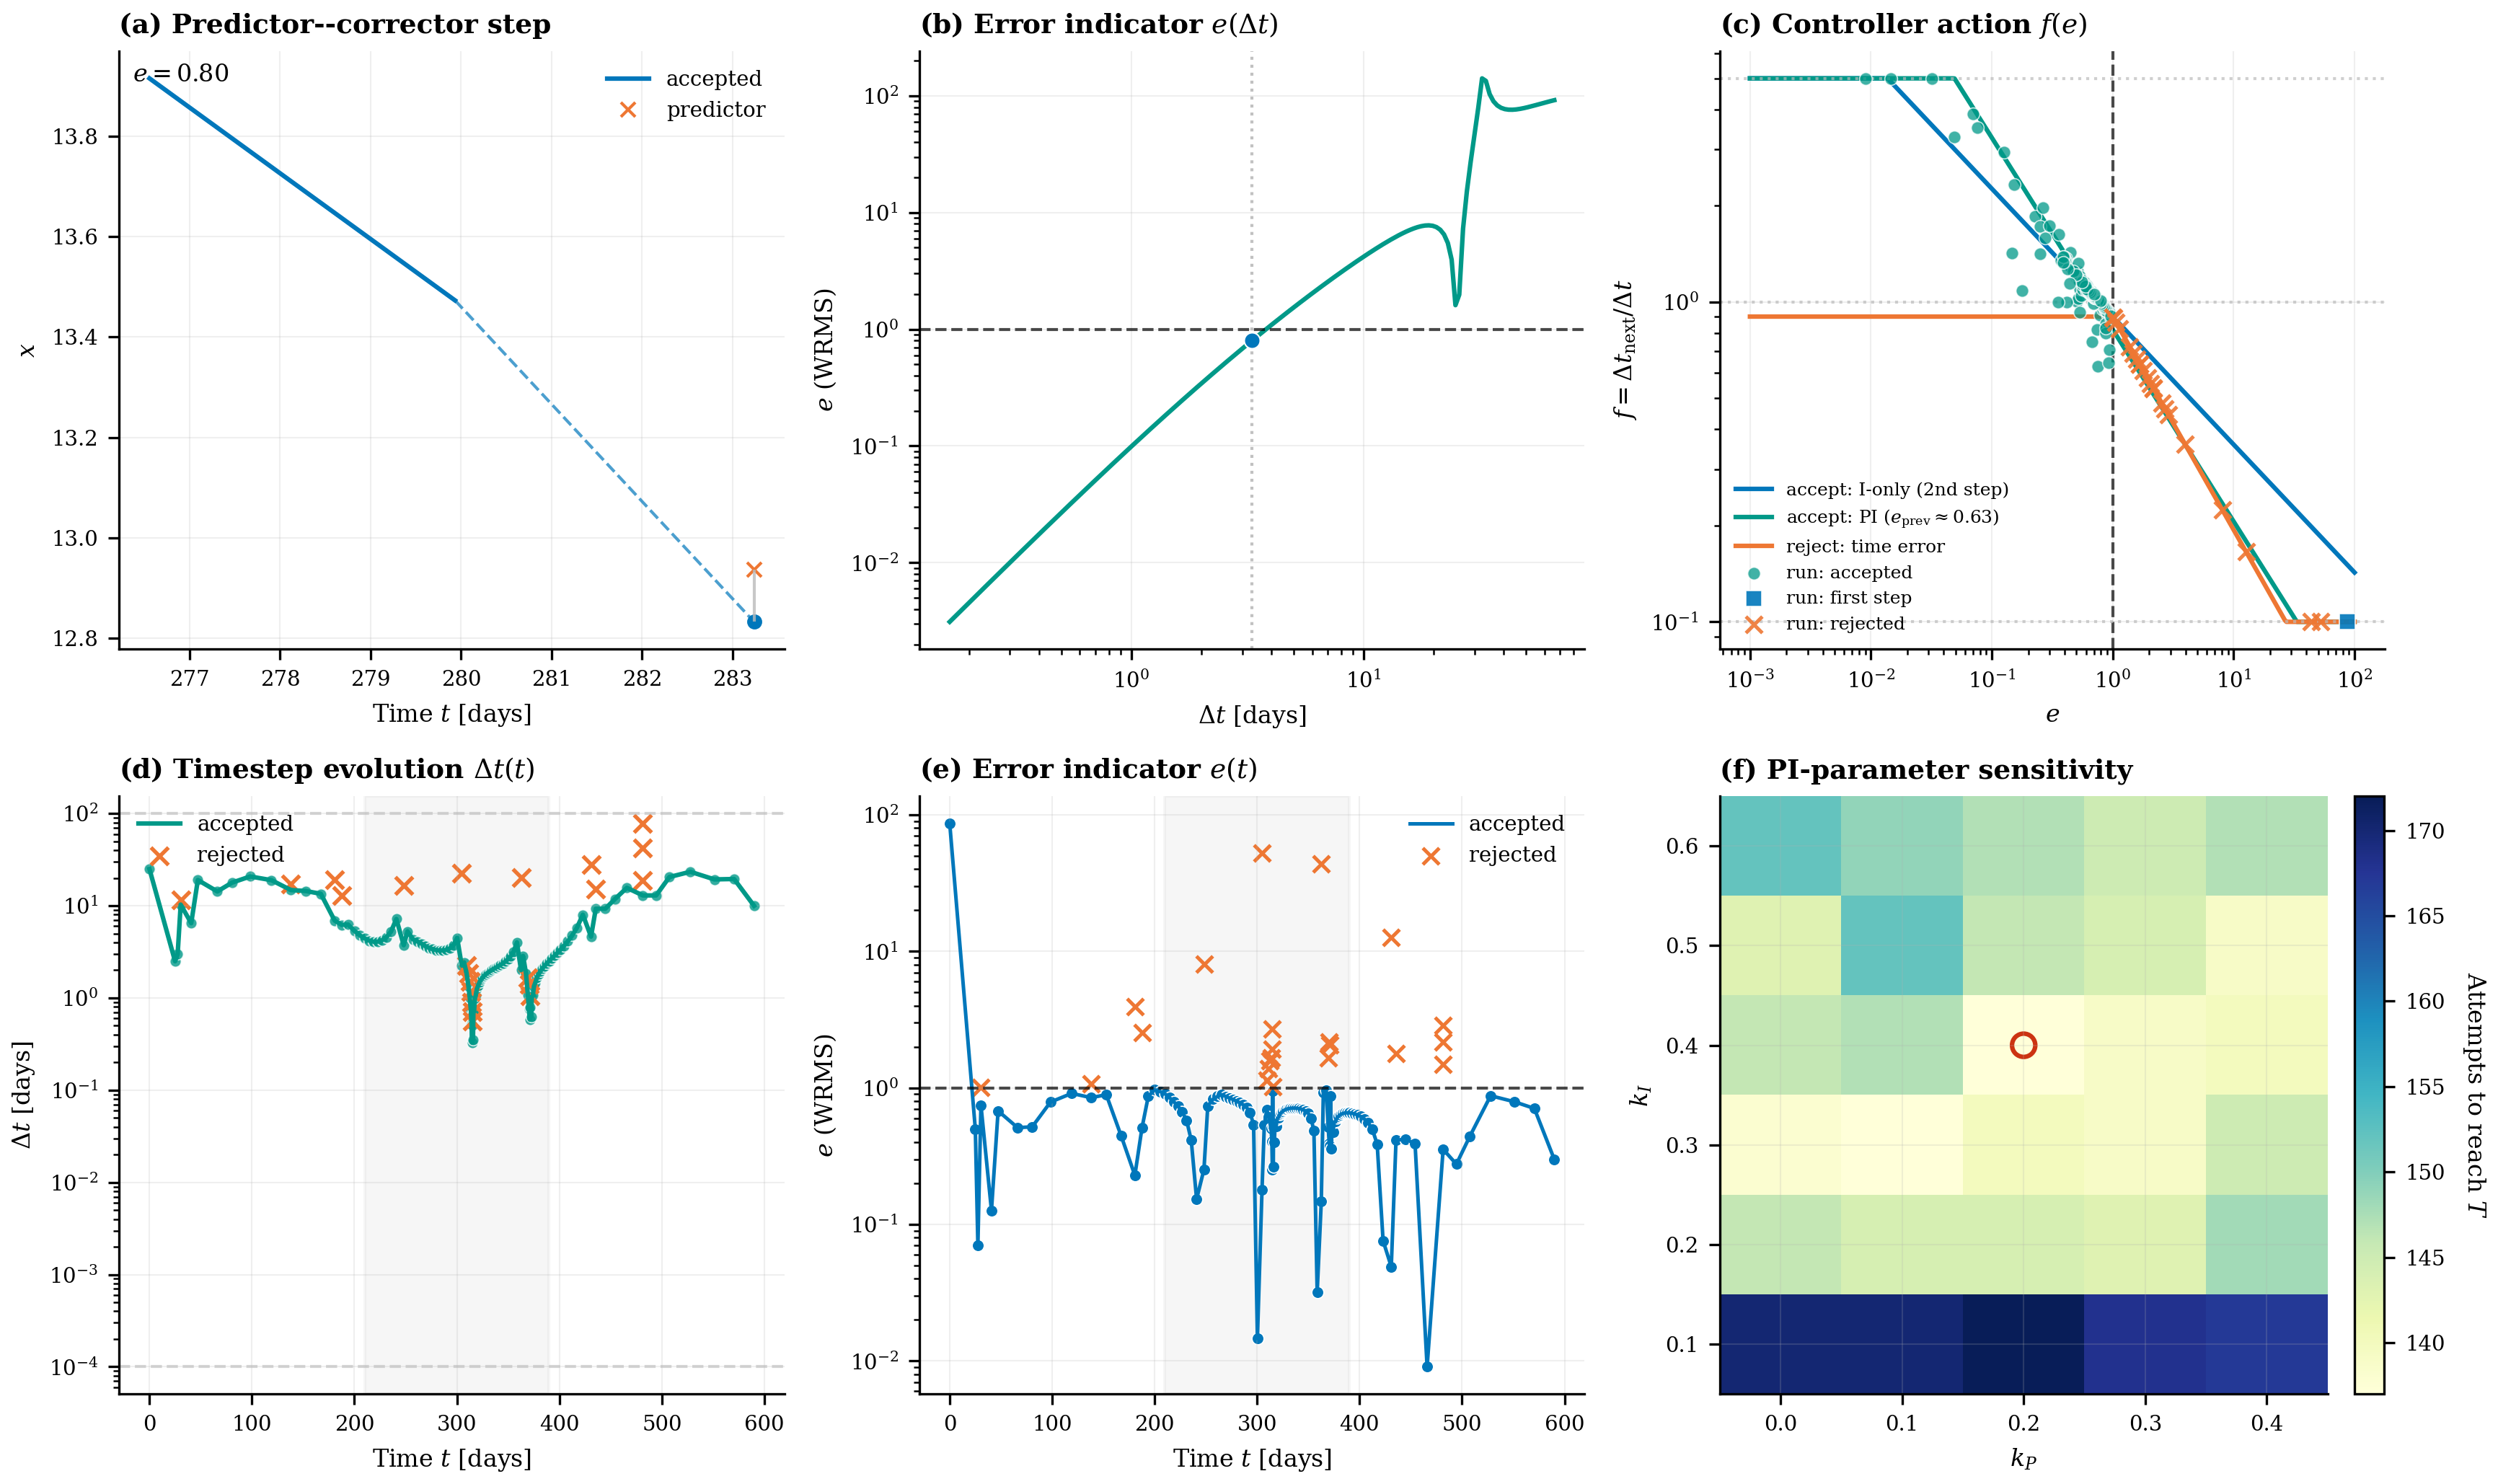
\includegraphics[width=1\linewidth]{images/time_adaptivity_demo.png}%
  }{\fbox{\parbox{0.9\linewidth}{\centering Missing image: \texttt{images/time_adaptivity_demo.png}}}}
  \caption{Analytic demonstration of the predictor--corrector error estimate and Gustafsson PI timestep controller (synthetic scalar ODE with a smooth transient forcing ``burst'' to trigger rejections). (a) One representative step: AB predictor $x_{\mathrm{pred}}^{n+1}$ and BE-corrected state $x^{n+1}$ define the WRMS error $e^{n+1}$. (b) Error indicator $e(\Delta t)$ for the same local history, with the selected timestep marked. (c) Controller action $f(e)=\Delta t_{\mathrm{next}}/\Delta t$ for accepted steps (I-only and PI) and for time-error rejections; markers overlay the actual $(e,f)$ pairs from the synthetic run. (d) Timestep evolution $\Delta t(t)$ and (e) the corresponding error history $e(t)$, with the acceptance threshold $e=1$. (f) Sensitivity of the total number of attempts to reach $T$ with respect to PI gains $(k_P,k_I)$.}
  \label{fig:time-adaptivity-controller}
\end{figure}

\paragraph{Output and mesh tags.}
We write field snapshots every $N_{\mathrm{save}}=1$ accepted timesteps and record per-step and per-subiteration solver telemetry. The Dirichlet and Neumann boundary parts $(\Gamma_D,\Gamma_N)$ are defined by mesh facet tags with IDs $(i_D,i_N)=(1,2)$.

\paragraph{Calibration for Convergence Studies.}
For the spatial convergence analysis presented in \ref{app:convergence}, we employ a box specimen with one face fixed and a compressive traction applied on the opposite face. The material parameters match the baseline set above, and all runs are advanced to the same final time to isolate discretization effects.

\subsection*{Preconditioner maintenance}\label{subsec:ksp_defaults}
Each subsolver keeps a single PETSc KSP object that is reused as $(\rho,\mathbf{L},S)$ evolve, with the operator updated after each assembly. Preconditioner setup therefore follows PETSc's standard reuse policy and is decoupled from the AA/GS logic.

% ==== End of clarifications ====
% --- ORIGINAL CONTENT ---
\subsection*{Anderson acceleration: convergence and diagnostics}
\label{subsec:anderson}
\paragraph{Motivation and scope}
To reduce the number of block fixed-point (block Picard/Gauss--Seidel) sub-iterations, we employ Anderson acceleration (AA) in the Pulay type-II (DIIS) form described in \S\ref{sec:fp-aa}, with finite memory $m$. We compare (i) a block Picard baseline (constant relaxation) and (ii) AA with step limiting and adaptive history restarts across representative couplings and time-step sizes $\Delta t$. We also report diagnostics that help choose~$m$ and monitor robustness.

\subsection*{Projected residual and stopping}\label{subsec:proj_merit}
We use the \emph{RMS-per-DOF} Picard residual $r_{\mathrm{Pic}}$ in \eqref{eq:fp-picard-res} on the flattened state $(\mathbf L,S,\rho)$ with the per-block scaling \eqref{eq:fp-scales}. The coupled solve stops when $r_{\mathrm{Pic}}\le \mathrm{tol}$ or when the maximum number of subiterations is reached. There is no per-iteration AA rejection/backtracking; robustness is provided by the step limiter \eqref{eq:aa-step-limit} and by history restarts based on conditioning and stall. Candidate formation follows \eqref{eq:aa-weights}--\eqref{eq:aa-update}.

\subsection*{Stacking vs.\ sweep order}\label{subsec:order}
The accelerated stacked state follows $(\mathbf L,S,\rho)$, while a single GS sweep updates blocks in the physical order \emph{mechanics driver} $\to$ fabric $\to$ stimulus $\to$ density (mechanics is recomputed inside the driver and is not part of the Anderson state).

\subsection*{Anderson acceleration details}\label{subsec:aa_details}
We employ the Pulay type-II (DIIS) Anderson scheme described in \S\ref{sec:fp-aa}. Specific settings for the results below include the step limit factor $c_{\mathrm{step}}$ and history depths $m$ as indicated in the figures. We restart the AA history upon (i) stagnation of $r_{\mathrm{Pic}}$ relative to the best value in a recent window, or (ii) poor conditioning of the regularized Gram system.

\paragraph{Performance diagnostics}
To assess stability and tuning, we monitor Anderson metrics over time and their sensitivity to $(\Delta t, m, \beta)$ (\cref{fig:aa-metrics}). At fixed $\Delta t=25$ days, a sliding-window view of the condition number $\kappa(H+\lambda_{\mathrm{eff}}I)$ remains well behaved across tested histories $m$ and mixing factors $\beta$. Aggregated over late-time windows, the timestep rejection rate stays moderate, the average history depth scales with $m$, and the median $\kappa(H+\lambda_{\mathrm{eff}}I)$ shows only mild growth with larger $m$ or $\beta$.

\begin{figure}[htbp]
  \centering
  \IfFileExists{images/anderson_performance_vs_time.png}{%
    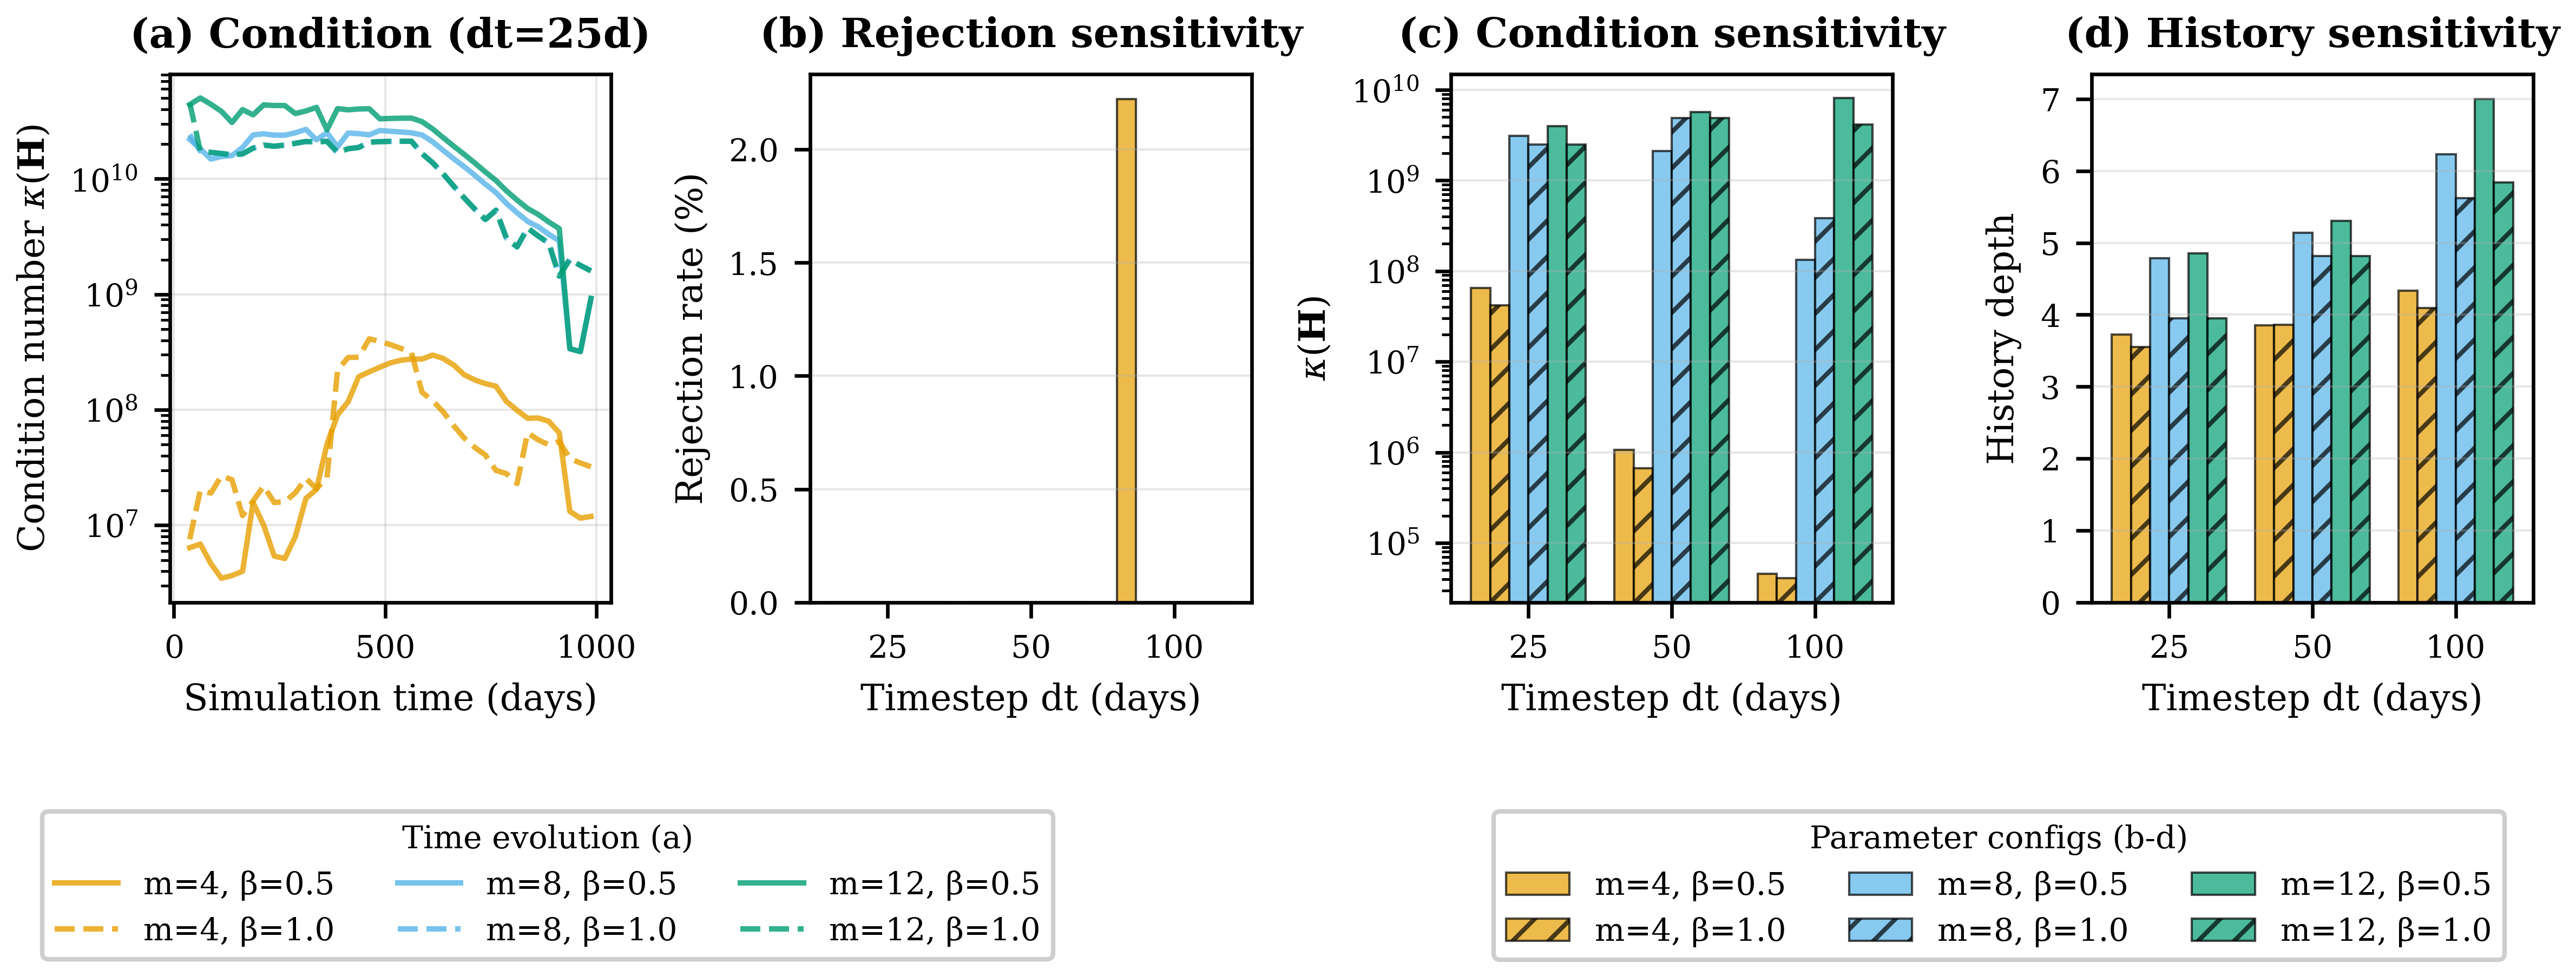
\includegraphics[width=1\linewidth]{images/anderson_performance_vs_time.png}%
  }{\fbox{\parbox{0.9\linewidth}{\centering Missing image: \texttt{images/anderson_performance_vs_time.png}}}}
  \caption{Anderson performance metrics and sensitivity. (a) Time-windowed condition number $\kappa(H+\lambda_{\mathrm{eff}}I)$ at fixed $\Delta t=25$ days for several $(m,\beta)$. (b) Timestep rejection rate (adaptive controller) averaged over the final window versus $\Delta t$, grouped by $(m,\beta)$. (c) Average $\kappa(H+\lambda_{\mathrm{eff}}I)$ (log scale) versus $\Delta t$. (d) Average Anderson history depth versus $\Delta t$.}
  \label{fig:aa-metrics}
\end{figure}

\paragraph{AA vs. Picard}
We compare the baseline block Picard scheme with Anderson acceleration across representative timestep sizes and coupling strengths (\cref{fig:aa-vs-picard}). In our runs, Anderson acceleration reduces sub-iterations per timestep and total walltime while preserving robustness via step limiting and history restarts; the benefit is largest in tighter couplings, with comparable behavior to Picard in mild regimes.

\begin{figure}[htbp]
  \centering
  \IfFileExists{images/anderson_vs_picard.png}{%
    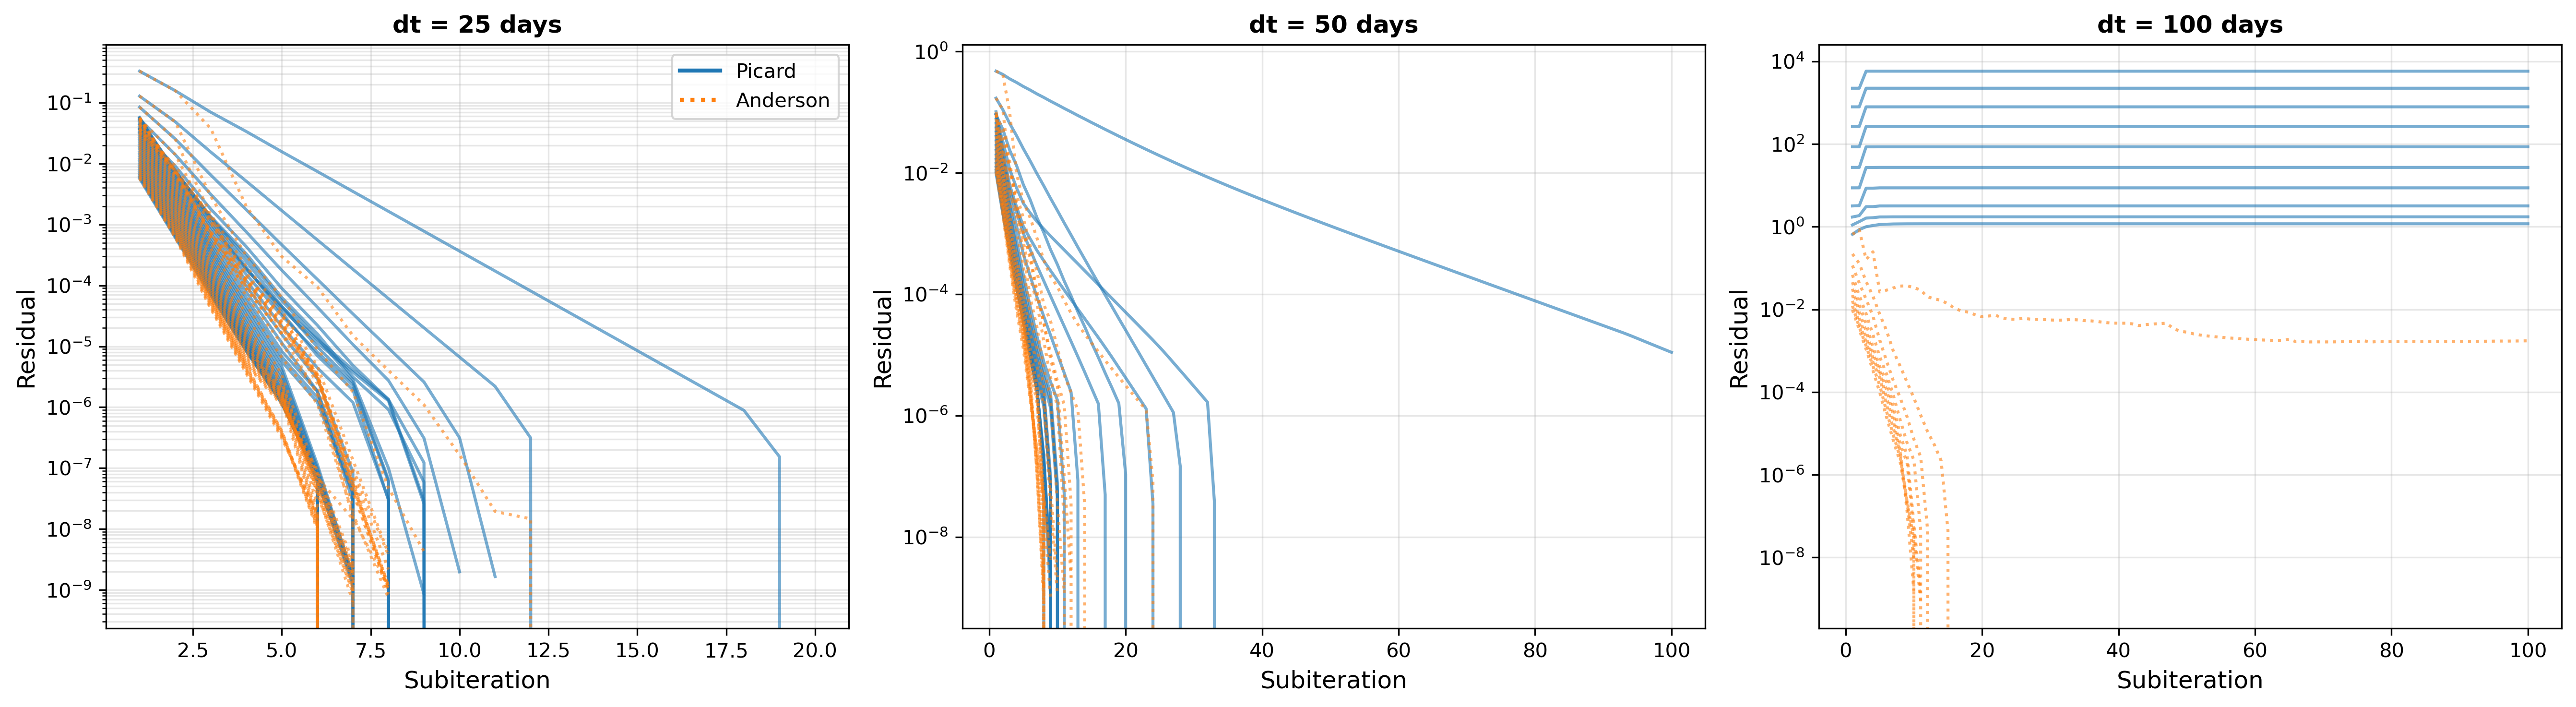
\includegraphics[width=1\linewidth]{images/anderson_vs_picard.png}%
  }{\fbox{\parbox{0.9\linewidth}{\centering Missing image: \texttt{images/anderson_vs_picard.png}}}}
  \caption{Comparison of block Picard and Anderson acceleration at representative $\Delta t$ and coupling strengths. Left: convergence behavior over time (projected-residual trends). Right: per-timestep subiterations and walltime summaries. Anderson acceleration reduces sub-iterations and computational cost while retaining robustness relative to Picard.}
  \label{fig:aa-vs-picard}
\end{figure}
